\documentclass{article}
\usepackage{spconf,amsmath,amssymb,graphicx,booktabs,array,microtype,dblfloatfix,float}
\graphicspath{{figures_icassp/}}
% Automatically generated from outputs/icassp_primary/summary.csv.
\newcommand{\PixelFisherRange}{0.277--0.520}
\newcommand{\CaseSpearmanRange}{0.890--0.966}
\newcommand{\NAURCRange}{0.024--0.092}
\newcommand{\RRRFiftyRange}{19.3--52.1\%}

% Automatically generated from outputs/shared_error_stress/summary.csv.
\newcommand{\StressMaeIncrease}{14.9\%}
\newcommand{\StressTargetIncrease}{28.6\%}
\newcommand{\StressSharedChange}{0.0\%}
\newcommand{\StressCommitteeMaeIncrease}{11.8\%}

\newcommand{\CrossScaleRhoRange}{0.871--0.937}
\newcommand{\CrossScaleNAURCRange}{0.052--0.098}
\newcommand{\CrossScaleRRRRange}{18.8--22.2\%}
\newcommand{\MatchedAdvantageRange}{-0.010--0.014}
\newcommand{\MedianMeanDelta}{-0.001 [-0.008, 0.008]}
\newcommand{\MedianSpreadDelta}{0.011 [-0.007, 0.031]}

\setlength{\textfloatsep}{6pt plus 2pt minus 2pt}
\setlength{\dbltextfloatsep}{6pt plus 2pt minus 2pt}
\setlength{\floatsep}{5pt plus 2pt minus 2pt}
\setlength{\intextsep}{5pt plus 2pt minus 2pt}
\setlength{\tabcolsep}{3.0pt}
\renewcommand{\arraystretch}{0.94}
% Use the reference-only fifth page efficiently without changing margins or font size.
\makeatletter
\let\oldthebibliography\thebibliography
\renewcommand{\thebibliography}[1]{%
  \oldthebibliography{#1}%
  \setlength{\itemsep}{0pt}%
  \setlength{\parsep}{0pt}%
  \setlength{\parskip}{0pt}%
}
\makeatother

\title{TARGET-TO-COMMITTEE DISAGREEMENT FOR MRI SLICE REVIEW:\\
SELECTION, TRANSFER, AND FAILURE BOUNDARIES}
\name{Anonymous Authors}
\address{Anonymous submission}

\begin{document}
\ninept
\maketitle

\begin{abstract}
Cohort-average fidelity cannot identify which MRI interpolation should be reviewed when the missing target is unavailable. We evaluate ground-truth-free ranking from deterministic outputs: a target interpolator is excluded from a heterogeneous committee, and its median target-to-member difference is aggregated over generated foreground voxels. Ground truth is isolated from scoring. We register 132 score--mask--pooling candidates and 40 score--committee combinations on IXI $\times4$ and fastMRI-brain $\times2/\times4/\times6$, freeze four finalists, and validate once on 22 eight-fold out-of-fold NingXia examinations at all factors. A development-selected committee reduces mean nAURC from 0.089 to 0.040 but degrades it from 0.070 to 0.116 on frozen validation. The pre-specified score remains strongest (Spearman 0.901, nAURC 0.070, RRR50 21.8\%). This transfer failure, paired bootstrap analysis, and common-mode decomposition show that committee selection can overfit cohort difficulty. Disagreement supports selective review, not calibrated uncertainty or clinical certification.
\end{abstract}

\begin{keywords}
MRI interpolation, reliability ranking, selective review, model disagreement, quality control
\end{keywords}

\section{Introduction}
Through-plane interpolation densifies sparse MRI stacks for visualization, registration, and volumetric processing. Modern methods model inter-slice context or adapt restoration transformers \cite{song2024i3net,liang2021swinir,chen2022hat}, yet they are usually compared by cohort-average PSNR, SSIM, or MAE. Such metrics summarize a test set but do not identify an unreliable examination once the missing slice is unobservable.

Model-internal uncertainty methods use stochastic inference, repeated training, heteroscedastic objectives, TTA, posterior reconstruction, or learned error prediction \cite{gal2016dropout,lakshminarayanan2017deepensembles,kendall2017uncertainties,wang2018tta,edupuganti2021uqmri,kuestner2024ensembles,shaw2020heteroscedastic,hu2021predict,zhang2024trainingfree}; no-reference MRI quality assessment instead targets perceptual quality or acquisition artifacts \cite{stepien2022nriqa}. Our setting assumes only deterministic outputs. Selective prediction supplies the endpoint \cite{elyaniv2010selective,geifman2019selectivenet,ding2020aurc,kompa2021second}. We contribute (1) a self-excluded target-to-committee ranking protocol and common-mode error boundary, (2) a registered candidate funnel with strict development/validation separation, and (3) a multi-factor transfer study showing that development-selected committees need not improve independent-cohort review.

\section{Method}
\subsection{Deployment contract and target isolation}
Let $x$ denote observed sparse-slice context, $y$ the unobserved dense target, and $\hat y_m=f_m(x)$ the output of target interpolator $m$. Available output identities form $\mathcal B$, and the target-specific committee is
\begin{equation}
 \mathcal C_m=\{\hat y_b:b\in\mathcal B,\ b\neq m\}.
 \label{eq:committee}
\end{equation}
The committee may combine neural point reconstructions with deterministic analytical interpolation, but never contains $y$ or $\hat y_m$ itself. Before scoring, outputs must share case identity, affine, orientation, voxel grid, shape, generated-slice pattern, and source-intensity representation. Missing, duplicate, non-finite, or geometrically mismatched files invalidate the profile rather than being silently resampled. Disagreement is meaningful only under this deployment contract.

\begin{figure}[!t]
 \centering
 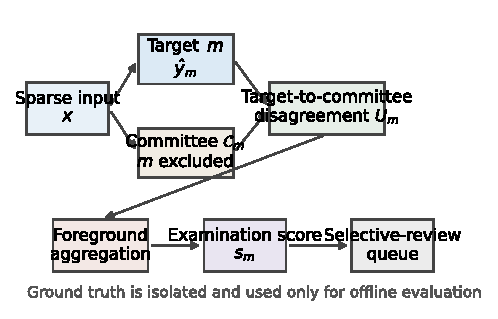
\includegraphics[width=0.98\columnwidth]{figure_framework_outlined.pdf}
 \caption{Target-specific scoring and offline evaluation. The target is excluded from its heterogeneous committee; ground truth is revealed only after scoring.}
 \label{fig:framework}
\end{figure}

\subsection{Target-specific disagreement family}
For generated voxel $i$, the default map is
\begin{equation}
 U_m(i)=\mathop{\mathrm{median}}_{b\in\mathcal C_m}
 |\hat y_m(i)-\hat y_b(i)|.
 \label{eq:score}
\end{equation}
This is a median target-to-committee difference, not statistical median absolute deviation and not posterior variance. Self-exclusion is essential because including $\hat y_m$ creates a structural zero. To separate the protocol from the elementary aggregator, define $d_{mb}(i)=|\hat y_m(i)-\hat y_b(i)|$ and
\begin{equation}
 U_m^g(i)=g\!\left(\{d_{mb}(i):b\in\mathcal C_m\}\right),
 \label{eq:family}
\end{equation}
where $g$ may be the median, mean, maximum, or trimmed mean. Comparators also include distance to the committee mean/median image, target-excluded committee spread, mean/median pairwise disagreement, residuals to linear/cubic interpolation, and gradient- or Laplacian-domain variants. These tests distinguish robust target conditioning from generic set dispersion, analytical departure, and local structural inconsistency. Changing the named target changes every $d_{mb}$ and may change the review order; a single all-output spread map cannot attribute risk to one interpolator.

\subsection{Generated support, masking, and intensity}
For factor $r$, let $\mathcal Z_{\rm obs}^{(r)}$ be the recorded anchor indices and $\mathcal Z_{\rm gen}^{(r)}=\mathcal Z\setminus\mathcal Z_{\rm obs}^{(r)}$. The audited runs begin at anchor $a=0$, hence $\mathcal Z_{\rm obs}^{(r)}=\{z:(z-a)\bmod r=0\}$; define $\mathcal G_r=\{i:i_z\in\mathcal Z_{\rm gen}^{(r)}\}$. Observed anchors are never scored. The default deployment mask and examination score are
\begin{align}
 M_m^{(r)}(i)&=\mathbf1\!\left[|\hat y_m(i)|>0.01\max_{j\in\mathcal G_r}|\hat y_m(j)|\right],\label{eq:mask}\\
 s_m^{(r)}&=\frac{\sum_{i\in\mathcal G_r}M_m^{(r)}(i)U_m(i)}{\sum_{i\in\mathcal G_r}M_m^{(r)}(i)}.
 \label{eq:case}
\end{align}
The formulation is independent of factor; $r$ only determines $\mathcal G_r$. Each factor forms a separate review queue because raw score scales need not be comparable. Foreground aggregation prevents background dominance, although a target mask may omit suppressed tissue. Ground-truth masks are rejected by the deployment path. Predictions share the source-volume intensity representation; independent output normalization is only a sensitivity because it can erase cross-model amplitude information.

\subsection{Identifiability and common-mode invariance}
Write $\hat y_b=y+c+\epsilon_b$, where $c$ is shared error and $\epsilon_b$ is member-specific. Then
\begin{equation}
 \hat y_m-\hat y_b=\epsilon_m-\epsilon_b.
 \label{eq:decomp}
\end{equation}
For any perturbation $c'$ applied identically to the target and every committee member on the evaluated support,
\begin{equation}
 U_m(\{\hat y_b+c'\})=U_m(\{\hat y_b\}),
 \label{eq:invariance}
\end{equation}
because each target-to-member difference is unchanged. This exact common-mode invariance is both the method's rationale and its blind spot: target-specific separation can be ranked, but shared deletion, blur, bias, or preprocessing failure is unidentifiable from disagreement alone. Committee diversity is therefore a necessary operating condition, not a guarantee that consensus is correct.

\subsection{Selective review and implementation separation}
Ground truth enters only offline. Let $E_j$ be foreground MAE for examination $j$. Sorting by increasing $s_m$ yields the retained set $A_q$ at coverage $q$ and risk
\begin{equation}
 R(q)=|A_q|^{-1}\sum_{j\in A_q}E_j.
\end{equation}
We report foreground pixel Pearson correlation, examination-level Spearman $\rho$, absolute retained MAE, $\mathrm{RRR}(q)=[R_{\rm random}-R(q)]/R_{\rm random}$, and
\begin{equation}
 \mathrm{nAURC}=\frac{\mathrm{AURC}-\mathrm{AURC}_{\rm oracle}}
 {\mathrm{AURC}_{\rm random}-\mathrm{AURC}_{\rm oracle}},
 \label{eq:naurc}
\end{equation}
where zero is oracle and one expected random review. Coverage is always the retained fraction; $1-q$ is referred. Only ordering is interpreted---the magnitude of $s_m$ is not an error probability. Computing Eq.~\eqref{eq:score} costs $O(|\mathcal G||\mathcal C_m|)$ and can stream members. The scoring API receives predictions and metadata only; ground truth, oracle ranking, and error-derived labels reside in a separate evaluator, preventing accidental leakage.

\section{Experiments}
\subsection{Cohorts, outputs, and frozen protocol}
The factor-four study uses IXI (115 examinations) \cite{ixi}, fastMRI-brain (24) \cite{zbontar2018fastmri}, and an internal NingXia cohort (22) pooled from eight held-out folds. IXI includes I$^3$Net, HAT, SwinIR, and ACSI; the other cohorts include the first three. Linear and cubic interpolation provide analytical references \cite{keys1981cubic,thevenaz2000interpolation,unser1999splines}, yielding 161 examinations and ten fixed profiles. The pre-declared cross-factor extension uses the identical fastMRI-brain and NingXia identities at $r\in\{2,4,6\}$ and freezes the common model set to I$^3$Net, HAT, SwinIR, linear, and cubic. A separate expanded sensitivity adds ArSSR, CycleINR, Pix2PixGAN, and SMamba-UNet only because all six aligned prediction sets exist; reconstruction fidelity was not used to select members.

\begin{table}[!t]
 \centering
 \caption{Cohorts and stored neural outputs. Analytical references are available for every profile.}
 \resizebox{\columnwidth}{!}{\begin{tabular}{lcll}
\toprule
Cohort & $n$ & Neural target outputs & Evaluation design \\
\midrule
IXI & 115 & I$^3$Net, HAT, SwinIR, ACSI & fixed held-out outputs \\
fastMRI-brain & 24 & I$^3$Net, HAT, SwinIR & fixed stored outputs \\
NingXia & 22 & I$^3$Net, HAT, SwinIR & eight-fold out-of-fold \\
\bottomrule
\end{tabular}
}
 \label{tab:protocol}
\end{table}

All NIfTI identities, geometry, and generated indices are checked before scoring. The frozen configuration uses all non-target members, Eq.~\eqref{eq:score}, raw inverse-normalized intensity, the 1\% target mask, and 2,000 paired examination-bootstrap resamples. The cross-factor seed is 20260724; matched cases reuse bootstrap identities. Every legal factor-four committee subset is recomputed from voxel outputs. No external-test result changes the score, mask, or committee.

SwinIR flip-TTA is evaluated only where matching four-view maps exist. Pixel correlation is calculated per examination and aggregated by Fisher $z$; case ranking uses Spearman $\rho$ with paired bootstrap intervals. Identical bootstrap indices are reused for paired comparisons. Mask variants that alter the foreground support are summarized by score-rank stability and endpoint-specific intervals rather than invalid paired differences against a changed MAE definition. Highest-MAE-decile AUROC/AUPRC is secondary because the two smaller cohorts contain only three positives per target. No profile or examination is removed after observing its score, and no sensitivity result replaces the frozen primary configuration on an external cohort.

\subsection{Primary association and selective review}
\begin{table}[!t]
 \centering
 \caption{All ten pre-specified profiles. Lower nAURC is better; coverage is retained fraction.}
 \resizebox{\columnwidth}{!}{\begin{tabular}{lcccc}
\toprule
Profile & Pixel $r_z$ & Case $\rho$ [95\% CI] & nAURC [95\% CI] & RRR$_{50}$ \\
\midrule
IXI/ACSI & 0.435 & 0.954 [0.925, 0.972] & 0.035 [0.018, 0.060] & 50.1\% \\
IXI/HAT & 0.512 & 0.966 [0.940, 0.980] & 0.024 [0.012, 0.042] & 49.6\% \\
IXI/I$^3$Net & 0.351 & 0.951 [0.922, 0.969] & 0.044 [0.024, 0.073] & 52.1\% \\
IXI/SwinIR & 0.520 & 0.965 [0.937, 0.980] & 0.025 [0.012, 0.044] & 49.5\% \\
\midrule
fastMRI/HAT & 0.328 & 0.916 [0.758, 0.962] & 0.067 [0.017, 0.176] & 19.7\% \\
fastMRI/I$^3$Net & 0.291 & 0.890 [0.713, 0.966] & 0.092 [0.029, 0.194] & 19.3\% \\
fastMRI/SwinIR & 0.363 & 0.931 [0.781, 0.978] & 0.061 [0.012, 0.150] & 20.5\% \\
\midrule
NingXia/HAT & 0.277 & 0.929 [0.790, 0.975] & 0.076 [0.016, 0.228] & 22.2\% \\
NingXia/I$^3$Net & 0.356 & 0.914 [0.769, 0.970] & 0.063 [0.016, 0.186] & 23.1\% \\
NingXia/SwinIR & 0.279 & 0.936 [0.807, 0.983] & 0.036 [0.007, 0.120] & 21.4\% \\
\bottomrule
\end{tabular}
}
 \label{tab:main}
\end{table}

Table~\ref{tab:main} shows moderate foreground localization (\PixelFisherRange) but strong examination ranking (\CaseSpearmanRange). Aggregation over generated foreground suppresses local noise and preserves between-case severity even when the map does not precisely identify each erroneous structure. nAURC is \NAURCRange; at 50\% retained coverage, referring the highest-score half lowers retained MAE by \RRRFiftyRange\ relative to random review. Confidence intervals are widest on fastMRI-brain and NingXia, so the continuous curves are more informative than a single threshold.

\begin{figure*}[!t]
 \centering
 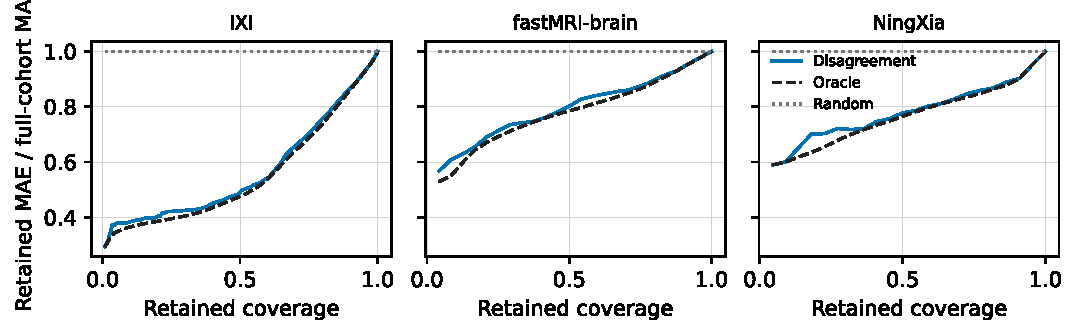
\includegraphics[width=0.82\textwidth]{figure_risk_coverage_outlined.pdf}
 \caption{Risk--coverage curves averaged over target interpolators after normalization by full-cohort MAE. The score remains between random and oracle review across cohorts; lower retained risk is better.}
 \label{fig:risk}
\end{figure*}

The complete curves in Fig.~\ref{fig:risk} avoid choosing a favorable test-set operating point. The largest absolute reduction occurs on IXI; smaller but consistent reductions occur on the two smaller cohorts. Because raw MAE is cohort-scale dependent, cross-cohort comparisons use nAURC and RRR rather than raw error.

\subsection{Score design, committee membership, and preprocessing}
\begin{table}[H]
 \centering
 \caption{Score and committee ablations averaged over fixed target profiles (nAURC; lower is better).}
 \resizebox{\columnwidth}{!}{\begin{tabular}{lll}
\toprule
Dataset & Score nAURC: med./mean/std. & Committee nAURC: neural/analytic/full \\
\midrule
fastMRI-brain & 0.073/0.070/0.074 & 0.017/0.118/0.073 \\
IXI & 0.032/0.043/0.049 & 0.033/0.059/0.032 \\
NingXia & 0.058/0.056/0.033 & 0.094/0.031/0.058 \\
\bottomrule
\end{tabular}
}
 \label{tab:ablation}
\end{table}

The median is a stable default but not a uniquely superior aggregator (Table~\ref{tab:ablation}). Across all 18 cross-factor profiles, its equal-profile $\Delta$nAURC versus mean is \MedianMeanDelta; versus target-invariant all-output spread it is \MedianSpreadDelta\ (negative favors median). Both intervals cross zero. The reliability signal is therefore not specific to the median, and target conditioning does not uniformly outperform generic examination difficulty. Committee composition is cohort dependent: neural peers are strongest on fastMRI-brain, analytical references on NingXia, and the full committee is near-best on IXI. Across legal factor-four subsets, nAURC spans 0.009--0.139; member identity matters more than size. The full committee is a frozen governance choice, not an empirical optimum.

Independent per-output normalization markedly degrades or reverses factor-four rankings, whereas input- and committee-derived masks largely preserve them. A common source-intensity representation is therefore part of the scoring contract; complete sensitivity results remain in the extended paper.

\subsection{Shared-error boundary and qualitative behavior}
The controlled stress test uses 20 fixed identity-sorted IXI examinations, all four targets, a foreground-constrained additive patch, five strengths, and a mask frozen before corruption. The target-specific arm perturbs only $\hat y_m$; the shared arm adds the identical patch to the target and every committee output.

\begin{figure}[!t]
 \centering
 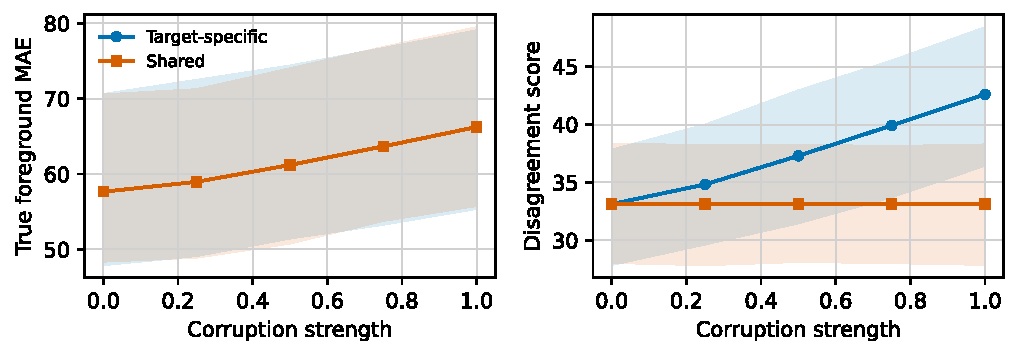
\includegraphics[width=0.98\columnwidth]{shared_error_stress_outlined.pdf}
 \caption{Controlled shared-error test. Target-specific corruption raises both MAE and disagreement; identical corruption of all outputs raises MAE while cancelling from target-to-member differences. Bands are 95\% bootstrap intervals.}
 \label{fig:stress}
\end{figure}

At maximum strength, target MAE rises by \StressMaeIncrease\ in both arms. Disagreement rises by \StressTargetIncrease\ for target-specific corruption but changes by \StressSharedChange\ under shared corruption, although mean committee MAE still rises by \StressCommitteeMaeIncrease. Figure~\ref{fig:stress} directly confirms Eq.~\eqref{eq:invariance}; it is an identifiability test rather than a simulation of all clinical failures.

\subsection{Cross-factor generalization and specificity}
Reconstruction MAE increases monotonically from $\times2$ to $\times6$ in both cohorts, but review ranking does not track difficulty monotonically. Target-averaged fastMRI-brain $\rho$/nAURC improves from 0.888/0.098 to 0.937/0.052. NingXia peaks at $\times4$ (0.926/0.058) and degrades at $\times6$ (0.871/0.097), while RRR50 remains 20.9\%; paired intervals do not establish degradation for every target. The complete plot and source data remain in the reproducibility package.

For direct target-specificity, we correlate each $s_m$ with every target model's true error. The matched-minus-mismatched advantage is only \MatchedAdvantageRange\ across six profiles, and every 95\% interval includes zero. The score ranks difficult examinations well but does not preferentially identify which of the three neural targets failed; shared case difficulty dominates. This negative result narrows the interpretation of ``target-to-committee'' from empirical attribution to an explicitly conditioned scoring construction.

\subsection{Single-model comparison and measured cost}
On the same 24 fastMRI-brain $\times4$ SwinIR examinations, four-view TTA yields $\rho=0.960$ and nAURC 0.023 versus 0.931 and 0.061 for committee scoring. The paired nAURC difference is $-0.038$ [95\% CI $-0.119$, 0.001], so the apparent gain is not conclusive. Stored-output auditing takes 1.18 s mean/2.87 s p95 per examination on CPU with 0.89 GiB peak RSS; online use additionally incurs every neural reconstruction.

\clearpage
\section{Extended Analyses}
\subsection{Registered candidate funnel and frozen validation}
The universal-bank audit verifies 11 neural and two analytical methods across fastMRI-brain and NingXia at factors two, four, and six. I$^3$Net, HAT, and SwinIR are the universal targets because they also exist on IXI. Development uses IXI $\times4$ and all fastMRI-brain factors; NingXia is not opened until four finalist definitions and their hash are serialized. Stage A evaluates 132 atomic score--mask--pooling candidates (74,052 case--target rows). Stage B combines five promoted definitions with eight committee policies, producing 40 score--committee candidates and 22,440 rows. Stage C uses 2,000 paired case-bootstrap resamples.

\begin{table}[H]
 \centering
 \caption{Frozen finalists on development profiles. Worst is maximum profile nAURC.}
 \resizebox{\columnwidth}{!}{\begin{tabular}{lcccc}
\toprule
Method & Mean nAURC & Worst & $\rho$ & RRR50 \\
\midrule
Pre-specified & 0.089 & 0.191 & 0.906 & 27.6\% \\
Low-cost & 0.087 & 0.159 & 0.906 & 27.8\% \\
Dev-selected universal & 0.040 & 0.099 & 0.947 & 28.1\% \\
Shared-difficulty & 0.036 & 0.093 & 0.952 & 28.1\% \\
\bottomrule
\end{tabular}
}
 \label{tab:optdev}
\end{table}

\begin{table}[H]
 \centering
 \caption{One-shot NingXia OOF validation averaged over three targets.}
 \resizebox{\columnwidth}{!}{\begin{tabular}{llccc}
\toprule
Method & Factor & $\rho$ & nAURC$\downarrow$ & RRR50$\uparrow$ \\
\midrule
Pre-specified & $\times$2 & 0.903 & 0.059 & 22.3\% \\
\addlinespace[1.5pt]
Dev-selected universal & $\times$2 & 0.797 & 0.130 & 18.4\% \\
\addlinespace[1.5pt]
Low-cost & $\times$2 & 0.912 & 0.059 & 21.5\% \\
\addlinespace[1.5pt]
Shared-difficulty & $\times$2 & 0.859 & 0.098 & 19.5\% \\
\addlinespace[1.5pt]
Pre-specified & $\times$4 & 0.927 & 0.058 & 22.2\% \\
\addlinespace[1.5pt]
Dev-selected universal & $\times$4 & 0.906 & 0.062 & 22.2\% \\
\addlinespace[1.5pt]
Low-cost & $\times$4 & 0.922 & 0.055 & 22.2\% \\
\addlinespace[1.5pt]
Shared-difficulty & $\times$4 & 0.899 & 0.075 & 22.2\% \\
\addlinespace[1.5pt]
Pre-specified & $\times$6 & 0.874 & 0.094 & 20.9\% \\
\addlinespace[1.5pt]
Dev-selected universal & $\times$6 & 0.812 & 0.154 & 19.2\% \\
\addlinespace[1.5pt]
Low-cost & $\times$6 & 0.846 & 0.127 & 19.9\% \\
\addlinespace[1.5pt]
Shared-difficulty & $\times$6 & 0.784 & 0.160 & 19.4\% \\
\bottomrule
\end{tabular}
}
 \label{tab:optval}
\end{table}

The development-selected universal committee (I$^3$Net, SAINT, SMamba-UNet, and Pix2PixGAN, with target exclusion) cuts mean nAURC from 0.089 to 0.040. It fails to transfer: validation nAURC is 0.116 versus 0.070 for the pre-specified baseline, and RRR50 is 19.9\% versus 21.8\%. The paired nAURC difference is +0.049 [95\% bootstrap interval $-0.038$, 0.244]. The low-cost analytical-anchor method is closer at 0.080 but is not demonstrably better. The shared/target decomposition chooses a fully shared score on development and also fails validation. No validation result is used to replace or revise a finalist.

\begin{figure}[H]
 \centering
 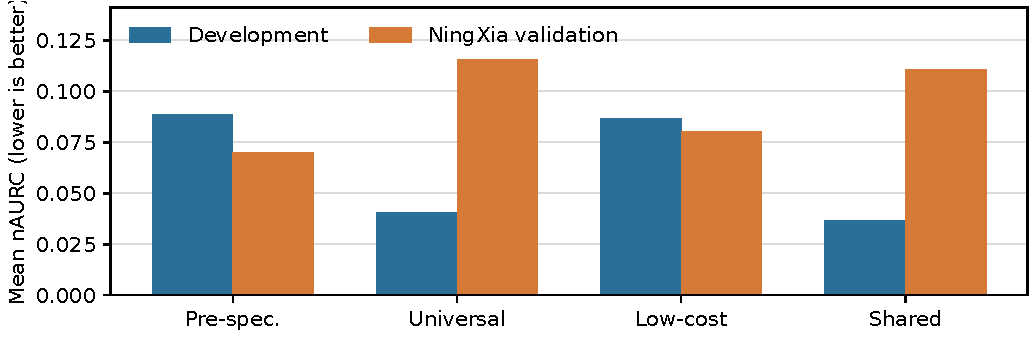
\includegraphics[width=\columnwidth]{figures_optimized/development_validation_transfer.pdf}
 \caption{Development-selected performance does not transfer to frozen NingXia validation. Lower nAURC is better.}
 \label{fig:opttransfer}
\end{figure}

Target-attribution matrices provide a second negative result. On NingXia, matched-minus-mismatched error correlation ranges from $-0.008$ to 0.014, usually with intervals containing zero. The construction is target-conditioned, but observed ranking mostly tracks shared examination difficulty. Cross-factor voxel consistency is not estimated because all 138 same-case comparisons have incompatible depth/generated support; defining a resampling rule after validation would violate the registered analysis.

\subsection{Reconstruction fidelity and expanded diversity}
Table~\ref{tab:fidelity} reports the original per-case reconstruction metrics from every model admitted to the expanded committee. All 42 dataset--factor--model rows were aggregated from the saved per-case CSV files; neither these metrics nor the resulting test errors were used to select the frozen primary committee. The added models span coordinate-based implicit reconstruction (ArSSR and CycleINR), adversarial convolutional synthesis (Pix2PixGAN), and a state-space/UNet hybrid (SMamba-UNet). Their availability allows a stricter diversity sensitivity than substituting one model at one factor.

\begin{table*}[!t]
 \centering
 \caption{Reconstruction fidelity for the seven neural outputs available at every factor. Metrics use each run's saved per-case generated-slice evaluation. Values are descriptive and were not used for committee selection.}
 \label{tab:fidelity}
 \begin{minipage}[t]{0.49\textwidth}
  \centering
  \textbf{fastMRI-brain}\\[2pt]
  \scriptsize
  \resizebox{\linewidth}{!}{\begin{tabular}{llrrrrr}
\toprule
Factor & Reconstructor & PSNR & SSIM & MAE & MSE & NCC \\
\midrule
$\times$2 & ArSSR & 23.11 & 0.761 & 43.6 & 8391.3 & 0.914 \\
$\times$2 & CycleINR & 23.10 & 0.759 & 43.7 & 8411.5 & 0.913 \\
$\times$2 & HAT & 24.65 & 0.811 & 37.3 & 6225.7 & 0.941 \\
$\times$2 & I$^3$Net & 27.77 & 0.867 & 25.3 & 3113.5 & 0.970 \\
$\times$2 & Pix2PixGAN & 26.07 & 0.830 & 31.2 & 4584.5 & 0.957 \\
$\times$2 & SMamba-UNet & 24.65 & 0.808 & 37.1 & 6361.1 & 0.940 \\
$\times$2 & SwinIR & 24.87 & 0.815 & 35.9 & 5990.4 & 0.943 \\
\addlinespace[2pt]
$\times$4 & ArSSR & 20.31 & 0.657 & 66.0 & 17745.9 & 0.830 \\
$\times$4 & CycleINR & 20.32 & 0.658 & 66.1 & 17743.2 & 0.830 \\
$\times$4 & HAT & 22.79 & 0.754 & 49.7 & 10454.5 & 0.908 \\
$\times$4 & I$^3$Net & 24.01 & 0.792 & 41.0 & 7755.7 & 0.931 \\
$\times$4 & Pix2PixGAN & 21.91 & 0.729 & 53.3 & 12485.2 & 0.891 \\
$\times$4 & SMamba-UNet & 22.73 & 0.762 & 49.4 & 10826.4 & 0.905 \\
$\times$4 & SwinIR & 22.36 & 0.745 & 52.0 & 11591.8 & 0.897 \\
\addlinespace[2pt]
$\times$6 & ArSSR & 19.42 & 0.616 & 74.9 & 21914.5 & 0.787 \\
$\times$6 & CycleINR & 19.39 & 0.616 & 74.9 & 22086.6 & 0.785 \\
$\times$6 & HAT & 21.82 & 0.731 & 55.8 & 13341.5 & 0.883 \\
$\times$6 & I$^3$Net & 22.83 & 0.762 & 47.1 & 10309.9 & 0.909 \\
$\times$6 & Pix2PixGAN & 21.65 & 0.725 & 54.8 & 13567.5 & 0.883 \\
$\times$6 & SMamba-UNet & 21.92 & 0.731 & 56.5 & 13166.7 & 0.885 \\
$\times$6 & SwinIR & 21.84 & 0.731 & 56.4 & 13267.8 & 0.884 \\
\bottomrule
\end{tabular}
}
 \end{minipage}\hfill
 \begin{minipage}[t]{0.49\textwidth}
  \centering
  \textbf{NingXia}\\[2pt]
  \scriptsize
  \resizebox{\linewidth}{!}{\begin{tabular}{llrrrrr}
\toprule
Factor & Reconstructor & PSNR & SSIM & MAE & MSE & NCC \\
\midrule
$\times$2 & ArSSR & 25.16 & 0.747 & 78.8 & 29980.4 & 0.911 \\
$\times$2 & CycleINR & 25.16 & 0.747 & 78.8 & 29980.4 & 0.911 \\
$\times$2 & HAT & 25.85 & 0.777 & 71.8 & 25723.3 & 0.924 \\
$\times$2 & I$^3$Net & 25.75 & 0.761 & 73.0 & 26688.8 & 0.923 \\
$\times$2 & Pix2PixGAN & 25.30 & 0.760 & 75.9 & 27897.9 & 0.915 \\
$\times$2 & SMamba-UNet & 25.45 & 0.764 & 76.7 & 28039.5 & 0.917 \\
$\times$2 & SwinIR & 25.58 & 0.768 & 75.3 & 27450.9 & 0.919 \\
\addlinespace[2pt]
$\times$4 & ArSSR & 23.21 & 0.714 & 98.3 & 41837.5 & 0.870 \\
$\times$4 & CycleINR & 22.94 & 0.698 & 103.3 & 44475.7 & 0.861 \\
$\times$4 & HAT & 23.99 & 0.755 & 87.8 & 35193.7 & 0.892 \\
$\times$4 & I$^3$Net & 23.48 & 0.724 & 96.1 & 39453.8 & 0.881 \\
$\times$4 & Pix2PixGAN & 22.44 & 0.716 & 108.0 & 51103.2 & 0.852 \\
$\times$4 & SMamba-UNet & 23.96 & 0.754 & 88.3 & 35445.0 & 0.891 \\
$\times$4 & SwinIR & 24.01 & 0.756 & 87.3 & 34871.0 & 0.892 \\
\addlinespace[2pt]
$\times$6 & ArSSR & 22.39 & 0.704 & 110.8 & 51461.2 & 0.836 \\
$\times$6 & CycleINR & 21.93 & 0.676 & 119.1 & 57033.3 & 0.818 \\
$\times$6 & HAT & 23.07 & 0.740 & 100.5 & 44299.8 & 0.862 \\
$\times$6 & I$^3$Net & 22.40 & 0.695 & 115.0 & 51157.7 & 0.843 \\
$\times$6 & Pix2PixGAN & 21.25 & 0.673 & 130.7 & 65474.6 & 0.801 \\
$\times$6 & SMamba-UNet & 23.01 & 0.737 & 102.8 & 45207.3 & 0.860 \\
$\times$6 & SwinIR & 23.04 & 0.740 & 100.6 & 44639.5 & 0.861 \\
\bottomrule
\end{tabular}
}
 \end{minipage}
\end{table*}

Adding all four diverse networks changes mean nAURC from 0.098 to 0.096 at fastMRI-brain $\times2$, from 0.073 to 0.088 at $\times4$, and from 0.052 to 0.050 at $\times6$. On NingXia, the corresponding changes are 0.065 to 0.110, 0.058 to 0.046, and 0.097 to 0.110. Thus broader architectural coverage is not monotonically beneficial: added members can sharpen consensus at one profile and dilute a useful analytical/neural contrast at another. This expanded analysis is intentionally labelled retrospective sensitivity and does not replace the five-member primary intersection.

The raw MAE scale is dataset specific, but within each cohort reconstruction difficulty rises with factor for every primary target. This trend does not force ranking quality to decline: reliability depends on whether difficult examinations create observable between-reconstructor separation, not only on mean reconstruction error. In particular, fastMRI-brain ranking improves as error grows, while NingXia $\times6$ shows the clearest scale-dependent degradation.

\subsection{Target specificity beyond shared case difficulty}
For each dataset and factor, Fig.~\ref{fig:matched} reports
\begin{align}
 R_{m,b}&=\operatorname{Spearman}(s_m,E_b),\\
 A&=\frac{1}{3}\sum_m R_{m,m}-\frac{1}{6}\sum_{m\ne b}R_{m,b},
 \label{eq:matched}
\end{align}
where $A$ is the matched-target advantage. The matrix is fixed at $3\times3$ because I$^3$Net, HAT, and SwinIR are common neural targets at every profile. Paired case bootstrap resamples all nine cells with identical case indices.

\begin{figure*}[!t]
 \centering
 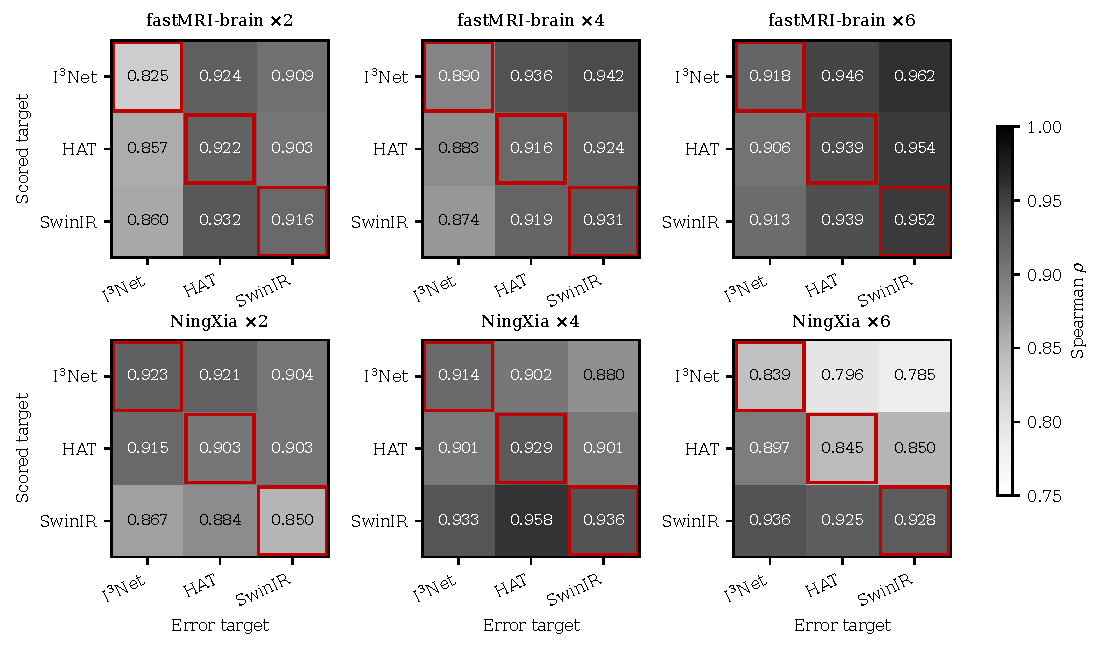
\includegraphics[width=0.72\textwidth]{matched_target_heatmap.pdf}
 \caption{Direct target-specificity test. Rows identify the score's named target and columns the model whose true error is correlated with that score. Red boxes mark matched cells. Similar within-row values show that shared examination difficulty dominates target identity.}
 \label{fig:matched}
\end{figure*}

\begin{table}[H]
 \centering
 \caption{Matched-target advantage from Eq.~\eqref{eq:matched}. Every interval includes zero.}
 \resizebox{\columnwidth}{!}{\begin{tabular}{llrr}
\toprule
Cohort & Factor & Matched advantage [95\% CI] & Row wins \\
\midrule
fastMRI-brain & $\times$2 & -0.010 [-0.036, 0.008] & 2/3 \\
fastMRI-brain & $\times$4 & -0.001 [-0.013, 0.008] & 2/3 \\
fastMRI-brain & $\times$6 & -0.000 [-0.017, 0.018] & 2/3 \\
NingXia & $\times$2 & -0.007 [-0.039, 0.007] & 1/3 \\
NingXia & $\times$4 & 0.014 [-0.001, 0.051] & 2/3 \\
NingXia & $\times$6 & 0.006 [-0.019, 0.033] & 1/3 \\
\bottomrule
\end{tabular}
}
 \label{tab:matched}
\end{table}

The six advantages range from \MatchedAdvantageRange, with only one or two of three diagonal cells exceeding their row's mismatched mean. The target-invariant all-output spread has exactly zero advantage by construction. Raw within-examination top-1 attribution is also unstable: it is 0\% on all fastMRI factors, 36.4\% on NingXia $\times2$, and 95.5\% on NingXia $\times4$/$\times6$. Score magnitudes therefore should not be compared across target identities without calibration. These results do not invalidate examination-level selective review; they invalidate the stronger interpretation that the score identifies which reconstructor is uniquely responsible for a difficult case.

\subsection{Paired comparator analysis}
Figure~\ref{fig:forest} uses the same bootstrap case identities for both members of each comparison. For method A equal to target median and method B the comparator, $\Delta\mathrm{nAURC}=\mathrm{nAURC}_A-\mathrm{nAURC}_B$; negative values favor the median. Equal-profile aggregates average the 18 fixed dataset--factor--target endpoints rather than pooling examinations across cohorts.

\begin{figure}[!t]
 \centering
 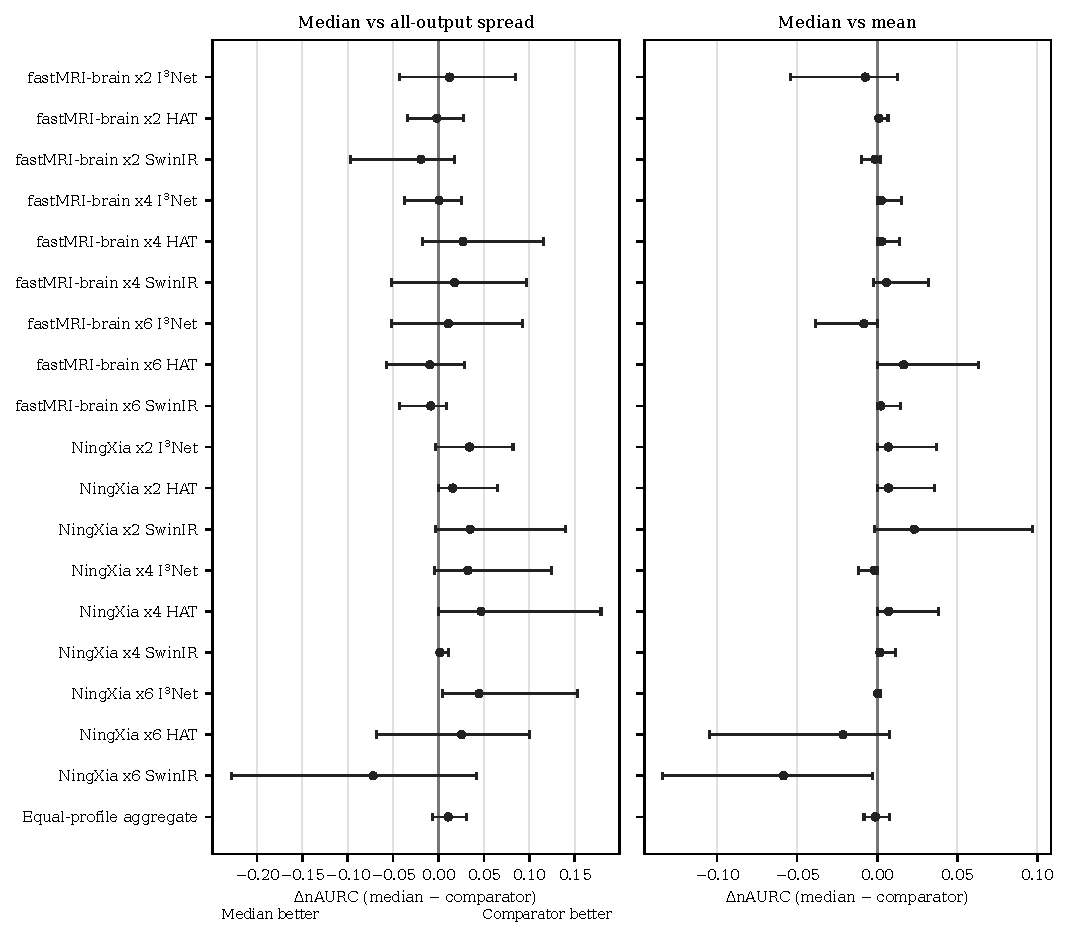
\includegraphics[width=\columnwidth]{paired_comparison_forest.pdf}
 \caption{Paired nAURC differences for every fixed cross-factor profile and the equal-profile aggregate. Intervals are 95\% paired case-bootstrap intervals. No profile was removed after observing its comparison.}
 \label{fig:forest}
\end{figure}

\begin{table}[!t]
 \centering
 \caption{Equal-profile paired comparisons; negative $\Delta$nAURC favors median.}
 \resizebox{\columnwidth}{!}{\begin{tabular}{lrr}
\toprule
Comparator & $\Delta$nAURC [95\% CI] & Profiles \\
\midrule
Mean target-to-member & -0.001 [-0.008, 0.008] & 18 \\
All-output spread & 0.011 [-0.007, 0.031] & 18 \\
Excluded-committee spread & -0.003 [-0.026, 0.020] & 18 \\
\bottomrule
\end{tabular}
}
 \label{tab:paired}
\end{table}

Median versus mean is effectively unresolved at the aggregate level (\MedianMeanDelta). Median is also not superior to all-output spread (\MedianSpreadDelta), and its difference from target-excluded spread is $-0.003$ [95\% CI $-0.026$, 0.020]. Full versus neural-only and analytical-only comparisons likewise vary by cohort and factor. We therefore retain the median as a pre-specified robust default, not as an empirically dominant algorithmic component. The contribution is the observable-output audit protocol, strict target exclusion, generated-support contract, selective-review evaluation, and explicit identification of what the score cannot establish.

\subsection{Sensitivity, failure examples, and deployment detail}
Independent p1--p99, median/IQR, or min--max normalization can destroy cross-model amplitude information and substantially worsen ranking. In contrast, committee-union, committee-intersection, committee-median, and observed-input masks mostly preserve examination ordering; high target thresholds are least stable on fastMRI-brain. The complete factor-four summary is retained in Table~\ref{tab:sensitivity_ext}.

\begin{table}[!t]
 \centering
 \caption{Factor-four sensitivity and secondary checks. Normalization columns report deterioration from raw intensity; mask entries are score-rank stability.}
 \resizebox{\columnwidth}{!}{\begin{tabular}{lll}
\toprule
Analysis & Result & Interpretation \\
\midrule
Normalization & $\Delta$nAURC $+0.248$--$+1.359$ & independent scaling degrades ranking \\
Mask stability & min. $\rho_s=0.606$; most $\geq0.973$ & robust except high fastMRI threshold \\
Legal subsets & nAURC $0.009$--$0.139$ & member identity matters more than size \\
SwinIR TTA & $0.023$ vs. $0.061$ nAURC & local gain inconclusive by paired CI \\
CPU audit & 1.18 s mean / 2.87 s p95 & stored-output post-processing only \\
\bottomrule
\end{tabular}
}
 \label{tab:sensitivity_ext}
\end{table}

Automatically selected failure examples complement the controlled common-mode experiment: a high-error examination can receive a low score when peers share over-smoothing, while a correct but unconventional detail can trigger unnecessary review. Highest-MAE-decile AUROC/AUPRC remains secondary because fastMRI-brain and NingXia contain only three positive examinations per target. Online deployment must additionally benchmark every neural member on matched hardware; the measured 1.18-s post-hoc time applies only when outputs already exist.

\begin{figure}[!t]
 \centering
 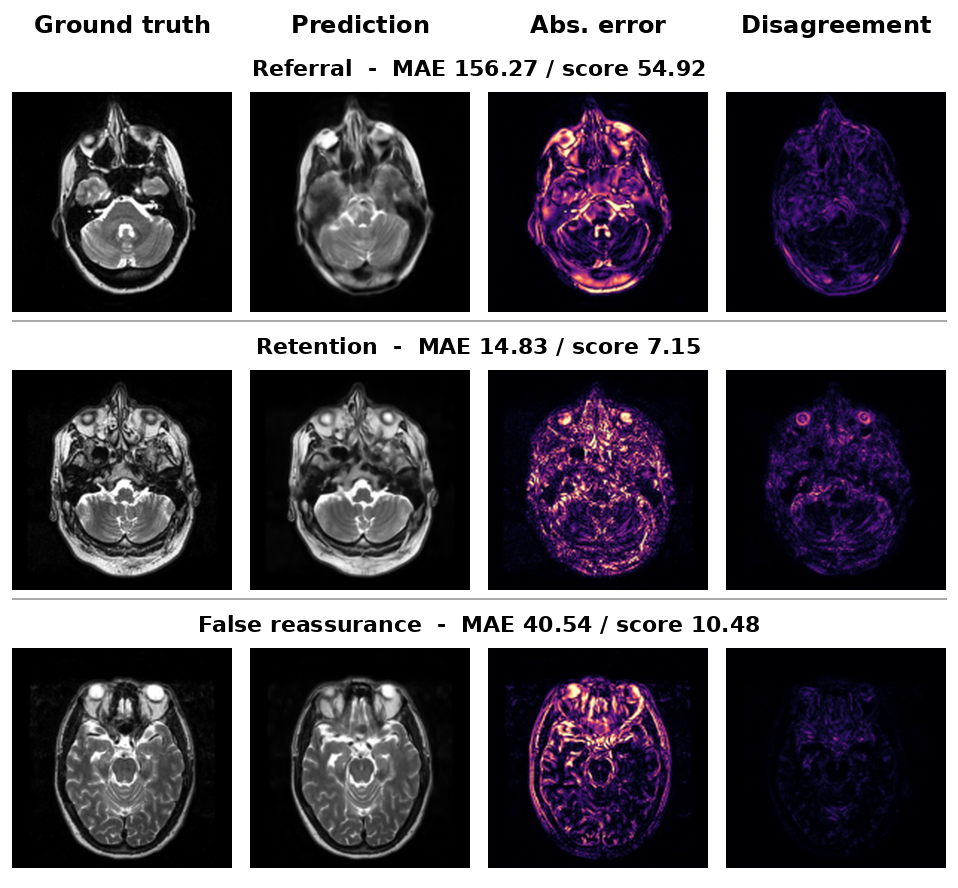
\includegraphics[width=0.98\columnwidth]{qualitative_failures_relayout.png}
 \caption{Automatically selected IXI/SwinIR examples: useful referral, stable retention, and false reassurance. Error is not interpreted as diagnostic harm.}
 \label{fig:qual_ext}
\end{figure}

\section{Discussion and Conclusion}
The evidence supports examination triage more strongly than precise voxel localization. A high $s_m$ prioritizes inspection while preserving the original reconstruction and committee identities; a low score indicates consensus only within the available committee. Coverage should follow review capacity rather than a retrospectively tuned error threshold, and a deployment threshold requires validation after changes in scanner, reconstruction software, intensity mapping, or committee membership.

The protocol is most attractive for retrospective audit, benchmark comparison, or systems that already cache several deterministic outputs. If only one model can be run, TTA, posterior sampling, acquisition residuals, or a validated error predictor may be more economical. A larger committee is not automatically better: member identity matters more than count, and the available no-reference diversity proxy cannot reliably choose the best compact subset. In practice, a review system should therefore freeze the committee specification, log member identities with every score, and monitor score distributions after software or acquisition changes rather than silently swapping members.

The score is also complementary to model-internal uncertainty. TTA probes sensitivity of one model to transformations, whereas cross-model disagreement probes separation from alternative reconstructions. Their failure modes need not coincide: one model may be unstable while peers agree, or all models may be confidently wrong together. A future deployment study should measure whether presenting both signals improves reviewer prioritization, review time, or downstream robustness without encouraging automation bias.

The principal limitations are structural. Shared errors are invisible, correlated members reduce diversity, a target mask can omit suppressed tissue, and unusual correct detail can be over-referred. Evidence remains restricted to T2 brain MRI; fastMRI-brain and NingXia are small, $\times6$ NingXia degrades, and the matched analysis cannot separate target identity from shared difficulty. There is no reader study or downstream task, and MAE is not diagnostic harm. Target-to-committee disagreement is therefore a reproducible ranking layer for selective review of stored outputs, not calibrated uncertainty, model attribution, or a clinical guarantee.

\clearpage
\bibliographystyle{IEEEbib}
\bibliography{references}
\end{document}
